The system was put through a series of tests using 14 different maps (examples in Appendix \ref{sec:app_04}) of varying sizes and levels of complexity. Each algorithm being evaluated is run on each map, with the agents' positions remaining tests runs with different algorithms. End-to-end test time is measured, from when the calculation is triggered by the agent until the final path is determined. Additional information such as how long it took to set up the test, any communication time, and how long the algorithm took to calculate the path can be found in the section \ref{sec:04_06_observability}. This allows for a thorough evaluation of the system's performance and helps identify any areas for improvement. Depending on the requirements, the system can be simulated in the cloud, run on an on-premises system, or even composed of virtual machines, those approaches are explained in further sections. For the final test, an approach with the real on-premises system is used to examine communication delay to system performance.

\subsection{System simulated in the cloud}
The system can be simulated in a cloud-based environment. This is achieved by creating and connecting multiple agents to the system through the utilization of multiple Kubernetes pods spawned in a separate namespace. The simulation of the agent is performed in a cloud environment, and as such, this scenario does not take into account any communication delays as all containers are communicating within a local network (cluster network). This approach allows for the simulation of a cloud-based environment while maintaining control over the test conditions and minimizing external variables that may affect the results. This scenario is particularly useful for testing the system's scalability and performance under a cloud-based deployment.

\subsection{Real system}
A small-scale system composed of three external devices (Raspberry Pi) was constructed to demonstrate the functionality of a real-world system. On each of these devices, an agent container was deployed. One of the devices serves as the host for the map-service and broker containers. This configuration is shown in the Figure \ref{fig:cluster}. This approach allows for the simulation of a real-world deployment scenario, while maintaining a manageable scale for testing and evaluation. This scenario is particularly useful for testing the system's functionality and performance under real-world conditions, as well as for evaluating the system's ability to integrate with external devices.

\begin{figure}[H]
    \centering
    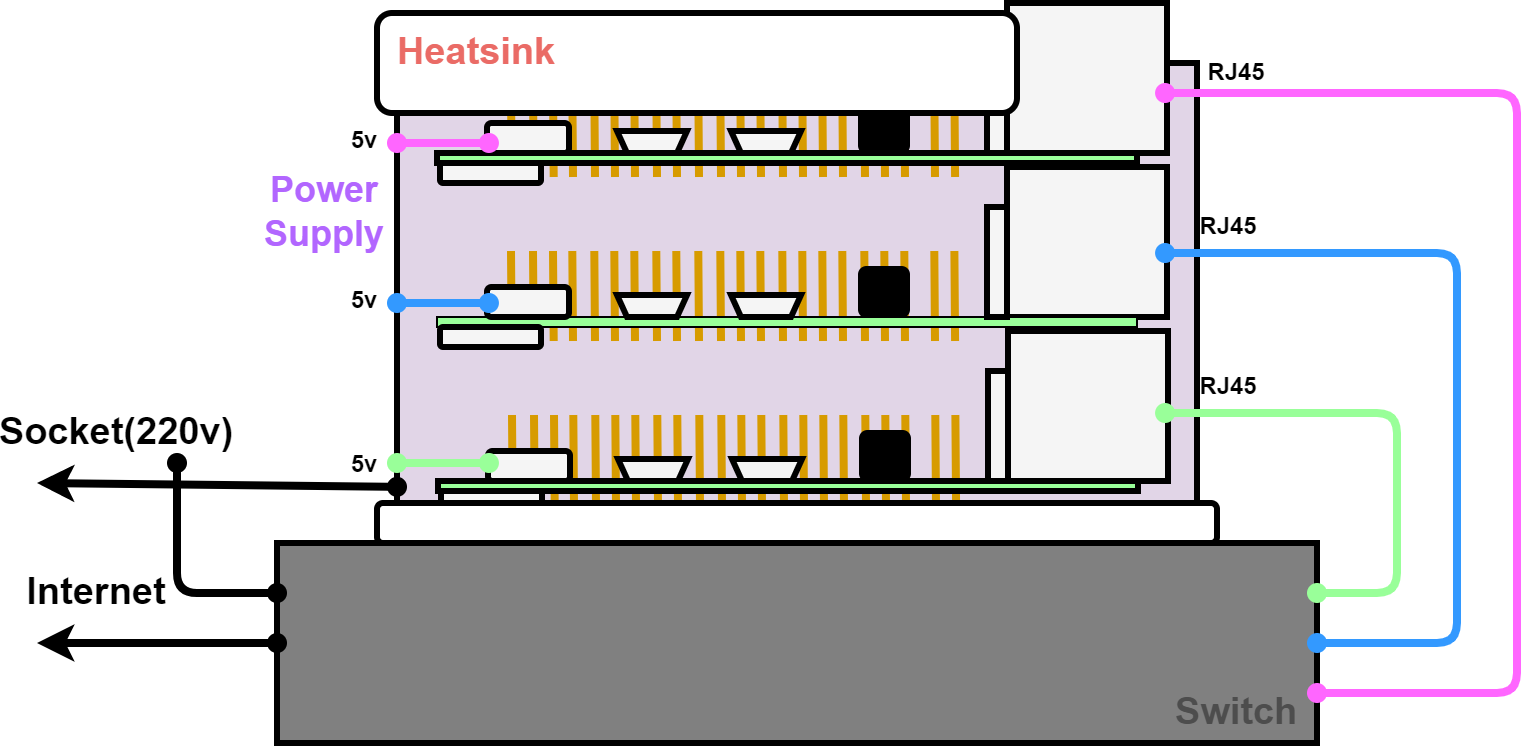
\includegraphics[width=0.8\textwidth]{pictures/cluster.png}
    \caption{Real cluster}
    \label{fig:cluster}
\end{figure}

This setup resembles a real-world scenario, with 3 robots (agents) and one server meant for deploying brokers and communicating to the cloud. Agents have limited resources as Single Board Computer used for deployment only has 1GB of memory and Quad-core Cortex-A72 1.5GHz processor \cite{rpi_specs}. For the purpose of the test, computing power can also be throttled. Devices are connected to the local network via an internet switch. 

The implementation of the solution presented a significant challenge due to the use of devices with ARM architecture. As a result, it was necessary to rebuild the containers to ensure compatibility with this architecture. To mitigate the difficulties associated with this process, the installation of Azure DevOps agents on the machines was implemented. This enabled the deployment of any software on the agent devices, and a Continuous Integration pipeline was put in place to rebuild ARM images on every code change using local machines as hosts and to push them into the image registry. Additionally, the cloud component of the solution was deployed on Okteto cloud, and both parts of the solution were able to exchange messages through the use of MQTT brokers. This approach ensured that the solution was robust and able to adapt to the unique technical requirements of the devices.

\subsection{System composed from virtual machines}
Another way of testing the system is to create a set of virtual machines or containers locally and connect them to the cloud system. The benefits of this approach are that this setup is easier to maintain, supports x86 architecture, and is easily extensible, as for spawning more agents there is no additional hardware needed. Resource limits can also be implemented both in the case of containers and virtual machines. Those entities have to be put in the same virtual network to enable communication between simulated machines.